% Sample document for SBGames papers
% Uses a slightly modified IEEE VGTC template in conference mode

\documentclass{vgtc}                          % final (conference style)

%% These three lines bring in essential packages: ``mathptmx'' for Type 1 
%% typefaces, ``graphicx'' for inclusion of EPS figures. and ``times''
%% for proper handling of the times font family.

\usepackage{mathptmx}
\usepackage{graphicx}
\usepackage{times}
\usepackage[utf8]{inputenc}

\usepackage{placeins}

%% We encourage the use of mathptmx for consistent usage of times font
%% throughout the proceedings. However, if you encounter conflicts
%% with other math-related packages, you may want to disable it.

%% If you are submitting a paper to a conference for review with a double
%% blind reviewing process, please replace the value ``0'' below with your
%% OnlineID. Otherwise, you may safely leave it at ``0''.
\onlineid{0}

%% declare the category of your paper, only shown in review mode
\vgtccategory{Research}

%% Paper title.

\title{TITLE}

%% Multiple authors with multiple affiliations:
\author{Thiago Santos Figueira$^{1}$
\and Adriano Mendes Gil$^{1}$}
\affiliation{\scriptsize $^{1}$Sidia Instituto de Ciência e Tecnologia
  (SIDIA)\\
  Manaus -- AM -- Brazil\\}

%% Abstract section.
%% Note how the keywords must be also included in this section!
\abstract{Virtual reality applications are very sensible to delay of synchronisation between user movements and its consequences on virtual environment. A way to accelerate the logic layer execution is to move its implementation to GPU. In this work we propose an architecture of visualization based on a shader parameterized by states and game elements positioning variables. As an example of this approach, we implemented a version of classic game Snake where every visual elements are defined and drawn by shader in an unique Mesh. Simultaneously, a way to mitigate inconsistencies during data reading in virtual reality joystick \textit{Gear VR Controller} through the Kalman filter is likewise described.

\smallskip

\noindent \textbf{Keywords:} Unity, Kalman filter, shaders, virtual reality games.
} 

%%%%%%%%%%%%%%%%%%%%%%%%%%%%%%%%%%%%%%%%%%%%%%%%%%%%%%%%%%%%%%%%
%%%%%%%%%%%%%%%%%%%%%% START OF THE PAPER %%%%%%%%%%%%%%%%%%%%%%
%%%%%%%%%%%%%%%%%%%%%%%%%%%%%%%%%%%%%%%%%%%%%%%%%%%%%%%%%%%%%%%%%

\begin{document}
\firstsection{Introduction}

\maketitle

%% do not uncomment this; use the \firstsection above
%%\section{Introduction} 
Virtual reality (VR) brings the promise of a revolution in the way entertainment is consumed in modern times. The user is placed at the center of the action and perceives content from every direction. Games, for their part,  transport players to a world envisioned by game developers and designers. As the technology for other form factors such as PC and console advances, VR players want life-like graphics and improved responsiveness. 

Regarding VR games development, Unity is the most used engine, and even though it is optimized, we believe there is an opportunity in exploring graphics cards for additional performance. Games developed in Unity follow a graphical pipeline where, generally speaking, the CPU (central processing unit) is responsible for transmitting graphics information to the GPU (graphics processing unit) through the Application stage, where the VRAM (video random access memory) loads graphics assets such as 3D models and textures. Afterward, during the Geometry stage, different objects and their information (positioning, for example) are handled by the GPU. The final stage, Rasterization, is where those objects become images.

%Highlight paper methodoloy

%Improve this section with proper references
The rest of this paper is structured as follows: the first section examines related works, the second one explores the designed architectures, the results section summarizes obtained results, and in the conclusions section we explore prospects for future work.

%-------------------------------------------------------------------------------------------------
\section{Related Works} \label{sec:relatedworks}
O jogo bidimensional \textit{GPGPUWars} \cite{GPGPUWars} utiliza uma estrutura baseada em \textit{shader} similar à arquitetura apresentada aqui onde a GPU executa todo o processamento do jogo criado. Contudo, aplicações em realidade virtual diferem-se de outras aplicações uma vez que há a necessidade de preencher o espaço tridimensional de forma a fornecer conteúdo para 3 graus de liberdade (3DoF - \textit{3 Degrees of Freedom}). Por exemplo, a aplicação descrita em \cite{zund2015unfolding} utiliza visão computacional para geração de uma visão panorâmica de um jogo de console em 8-bits. Rodando em um \textit{Oculus Rift DK2}, o dispositivo de realidade virtual do \textit{Facebook}, o jogador é posicionado no centro do mundo e à medida que movimenta seu personagem, o mundo é revelado ao seu redor, estendendo a visão de jogo para as quatro paredes do ambiente virtual.

Jogos VR são um grande potencializador de imersão, dada a sua capacidade de estimular a sensação de presença espacial e interatividade \cite{seibert2017control} através, por exemplo, dos controles \textit{VR} como o modelo ET-YO32 da Samsung, que são classificados como de mapeamento natural tangível realístico e consoante a definição proposta por \cite{skalski2011mapping}, emulam de forma realista sua contrapartida no ambiente virtual, ou seja, movimenta-se a réplica do controle físico no espaço 3D da aplicação VR da mesma forma que se faz no mundo real.

% 4 - Exemplos de filtragem de açoes dos controles (From ERIN17 paper. Refrasear)
Certos trabalhos trazem a filtragem de sensores baseados no uso de acelerômetro, a exemplo: \cite{schlomer2008gesture} usa o modelo oculto de Markov para reconhecimento de gestos em um controle do \textit{Nintendo Wii}, a filtragem ocorre por meio de filtros simples para remover pontos que não são suficientemente expressivos. \cite{shiratori2008accelerometer}, por outro lado, utilizam múltiplos controles de \textit{Nintendo Wii} para gerar animações proceduralmente, o ruído é atenuado através do uso do filtro de Kalman.

%-------------------------------------------------------------------------------------------------
\section{VRSnake} \label{sec:vrsnake}
% Definição das regras do jogo
\textit{VRSnake} brings to virtual reality the classic 2D game Snake, but unlike the original, the player establishes the positioning of the collectible objects rather than directly controlling the serpent. We then propose the following rules: 

The snake continuously and automatically seeks the collectible objects and grows in a unit as it reaches this object.

When the serpent reaches the boundaries of the scenario on one side, it continues the movement in the same direction on the other side. The player wins when the snake is defeated, that is when it hits itself in some way.

The exploration behavior of the snake must ensure there is no motion towards its body but likewise, guarantee randomization during movement to provide unpredictability.
%-------------------------------------------------------------------------------------------------

\section{Shader-based visualization architecture}
 \label{sec:architecture}
There are two approaches to the game architecture: in the first one, we use two layers of the graphics pipeline, and in the second one, we use a single layer.

In the first approach, one layer is responsible for handling the logic of the game, and the other is accountable for managing the rendering.  

The logical layer controls intelligent tasks such as the search for the collectible objects and movement furthermore it is executed in the Central Processing Unit (CPU) in CSharp.

The visualization layer involves shader, a piece of code that runs directly in the Graphics Processing Unit (GPU), which is responsible for rendering all items displayed on the output device, which includes the collectible objects as well as the snake.

In other words, the logical layer manages the collision and movement of the snake as well as selects the most promising path given a randomization factor; The visualization layer, on the other hand, is responsible for rendering all the elements arranged in the output device, that is, the CPU has no influence over these objects.

%-------------------------------------------------------------------------------------------------
\section{Realidade Virtual em uma Esfera Invertida} \label{sec:invertedsphere}

A ilusão em um mundo virtual e consequente sensação de imersão requerem material visual disponível em todos os ângulos possíveis, uma vez que o \textit{gearVR} possibilita completa liberdade de rotação, ou seja, 3 graus de liberdade (3DoF - \textit{3 Degrees of Freedom}). Tendo em vista que a proposta deste artigo contempla um jogo essencialmente 2D, tal como o \textit{Snake} original, tem-se o desafio de exibir conteúdo bidimensional em um cenário 3D de forma que tudo aconteça ao redor do usuário.

Uma esfera invertida, ou seja, uma esfera que tenha apenas seu lado interno renderizado, possibilita preencher completamente todo o campo de visão possível, além de ser a solução padrão adotada na exibição de imagens equiretangulares em 360 graus. A geração procedural de uma esfera pode seguir uma das duas abordagens abaixo:
\begin{enumerate}
  \begin{item} uma icosfera, i.e., uma esfera cujos vértices são distribuídos uniformemente; \end{item}
  \begin{item} geração de vertíces baseada em coordenadas de longitude/latitude. \end{item}
\end{enumerate}

Para este trabalho, preferiu-se a segunda abordagem devido a possibilidade de usar a longitude/latitude como forma de mapear as coordenadas de UV através da conversão abaixo:

\begin{equation}
R^2 \leftarrow R^3 : (\lambda, \theta) \rightarrow (x, y, z)
\label{equation1}
\end{equation}

% 2 - Mapeamento de UV em uma esfera invertida
Para calcular as posições dos vértices da esfera, dada uma quantidade de valores de latitude $N_{latitude}$ e uma quantidade de valores de longitude $N_{longitude}$, define-se um valor $R_{longitude}$ como o tamanho angular de longitude de uma secção transversal da esfera, tal como visto na equação \ref{equation1}.

\begin{equation}
R_{longitude} = \frac{2 \pi}{N_{longitude}}
\label{equation1}
\end{equation}

O tamanho angular total de uma quantidade de $i$ de valores de longitude pode ser dada pela equação \ref{equation2}.

\begin{equation}
\alpha_{i} = i * R_{longitude}
\label{equation2}
\end{equation}

Nas equações \ref{equation3} e \ref{equation4} definem-se as posições X e Z de pontos da esfera pertencentes a uma secção transversal da esfera que possui raio $D$.

\begin{equation}
x_{i} = D * \sin(\alpha_{i})
\label{equation3}
\end{equation}

\begin{equation}
z_{i} = D * \cos(\alpha_{i})
\label{equation4}
\end{equation}

Em um corte longitudinal, é possível perceber que o raio $D$ da secção transversal é variável ao longo da altura da esfera. Determina-se então um valor $R$ como o tamanho angular de um valor de latitude da esfera, tal como visto na equação \ref{equation5}.

\begin{equation}
R_{latitude} = \frac{\pi}{ N_{latitude}}
\label{equation5}
\end{equation}

O tamanho angular total de uma quantidade de $i$ de valores de latitude pode ser dado pela equação \ref{equation6}.

\begin{equation}
\alpha_{latitude} = i * R_{latitude}
\label{equation6}
\end{equation}

A posição Y dos pontos da esfera, considerando raio unitário, pode ser dada pela equação \ref{equation7}.
\begin{equation}
y_{i} = \cos(\alpha_{latitude})
\label{equation7}
\end{equation}

O raio $D_{yi}$ obtido em uma secção transversal na latitude $i$ é definido na equação \ref{equation8} como:
\begin{equation}
D_{yi} = 2 * \sin(\alpha_{yi})
\label{equation8}
\end{equation}

Aplicando-se a equação \ref{equation8} nas equações \ref{equation3} e \ref{equation4} obtém-se as posições X e Z dos vértices da esfera em função de suas coordenadas de longitude e latitude.

\begin{equation}
x_{i} = 2 * \sin(\alpha_{latitude}) * \sin(\alpha_{longitude})
\label{equation9}
\end{equation}

\begin{equation}
z_{i} = 2 * \sin(\alpha_{latitude}) * \cos(\alpha_{longitude})
\label{equation10}
\end{equation}

%-------------------------------------------------------------------------------------------------
\section{Snake como um Agente Utilitário} \label{sec:agent}

A inteligência de movimentação da \textit{snake} é, por sua vez, composta por uma função utilitária de avaliação de estados que analisa cada possível ação em determinado momento. Em essência, a serpente sempre está buscando alcançar o coletável, por isso avalia o curso de menor distância no eixos X e Y no espaço UV e desde que não exista a possibilidade de atingir a si própria, assume este caminho e repete o processo. A função abaixo ilustra esse procedimento:

\begin{equation}
F(A) = R * (D + O)
\label{equation11}
\end{equation}

Onde R é um fator de randomização; D representa a distância de \textit{Manhattan} entre a posição atual e o objeto coletável; e O é um valor atribuído à existência ou não de obstáculos neste trajeto.

A lógica de movimentação consiste em gerenciar o posicionamento da cabeça e corpo da serpente.  Em outras palavras, a cabeça norteia todo o movimentar da \textit{snake}, pois nela são traçados três vetores responsáveis por orientar a serpente na decisão do menor caminho entre sua atual posição e o objeto coletável. É relevante explicitar que estes vetores de direcionamento são volúveis tendo em vista as diferentes posições adotáveis.

O corpo da serpente, por sua vez, move-se através de um \textit{buffer} deslizante: cada parte do corpo assume a posição mais recente da parte imediatamente anterior, isso significa que a cabeça move-se e as demais partes seguem posteriormente.

%-------------------------------------------------------------------------------------------------
\section{Uso do Controle VR com Filtro de Kalman} \label{sec:gearvrcontroller}

Devido à natureza do jogo desenvolvido, o jogador necessita controlar o posicionamento do objeto coletável e para tanto existem essencialmente duas formas de interação num dispositivo de realidade virtual: o HMD (\textit{head-mounted display}), ou seja, através do sensor lateral acoplado ao próprio dispositivo; e os controladores externos, como os controles ou \textit{joysticks}. Em sua condição de sensor, porém, estes controladores estão sujeitos à interferência ruidosa durante a virtualização do evento representado no mundo real pelo movimento do usuário. Com a finalidade de melhorar a captura do sinal e traduzir de maneira mais fiel as intenções do jogador, o filtro de Kalman será aplicado às leituras do \textit{joystick} por meio de um componente de visualização de ruídos e aplicação do filtro

Para a efetiva implementação do filtro de Kalman na leitura do controle de realidade virtual seguem-se os seguintes passos: inicialmente captura-se a orientação angular do \textit{joystick}, traça-se um raio da posição virtual atual do controle até uma esfera unitária e o ponto resultante da interseção é o foco do usuário, em outras palavras, o objetivo apontado pelo cursor, esta posição é onde aplica-se o filtro de Kalman, proveniente da implementação encontrada na aplicação de \cite{KalmanComponent}.

%-------------------------------------------------------------------------------------------------
\section{Resultados} \label{sec:results}

Desenvolveu-se em realidade virtual o jogo \textit{Snake} no ambiente de desenvolvimento \textit{Unity}. Gerou-se uma aplicação \textit{android} testada no \textit{Samsung Galaxy S8} através do \textit{GearVR} com o controle de modelo ET-YO32. A figura \ref{fig:VRPerformanceChart} abaixo ilustra a taxa de quadros no \textit{GearVR} através da ferramenta de avaliação de performance da \textit{Oculus}, o \textit{OVR Metrics Tool}:

\begin{figure}[h!] 
\centering
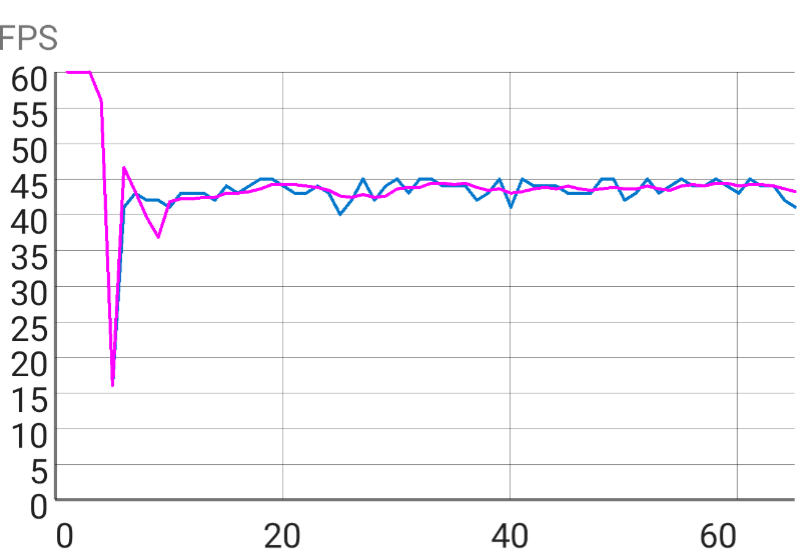
\includegraphics[width=\linewidth]{VRPerformance}
\caption{Quadros-por-segundo conforme o OVR Metrics Tool executado durante o funcionamento da aplicação }
\label{fig:VRPerformanceChart}
\end{figure}

A aplicação apresentou taxa média de 43.96 \textit{fps} (\textit{frames-per-second}, quadros-por-segundo), com mínima de 16 \textit{fps} e máxima de 60 \textit{fps}. Conforme representado pela figura \ref{fig:VRPerformanceChart}, a aplicação não mantém estáveis 60 \textit{fps} e isto se deve principalmente ao \textit{garbage collector} e à possíveis otimizações em código de GPU.

Durante a execução da aplicação, percebeu-se que quando a movimentação do cursor é mais veloz que a taxa de atualização, i.e., o \textit{update}, os pontos de ruído não são visualizados de maneira contínua, provocando o efeito visto na figura \ref{fig:filter02}, onde as partículas concentram-se em apenas alguns pontos amostrados pelo \textit{framerate} da aplicação \textit{Unity}, gerando regiões ruidosas espaçadas entre si.

Na figura \ref{fig:filter01} e \ref{fig:filter02} verifica-se que a linha azul forma-se de maneira estável ao longo do caminho percorrido pelo cursor, enquanto os pontos vermelhos se espalham ao redor desse caminho, indicando que a amplitude máxima de instabilidade é cerca de duas vezes maior que o tamanho do cursor, ou seja, facilmente perceptível pelo usuário e que impossibilitaria a realização de movimentos precisos e estáveis, em outras palavras, a exatidão e responsividade esperadas do controlador não são satisfatórias.

\begin{figure}[h!]
\centering
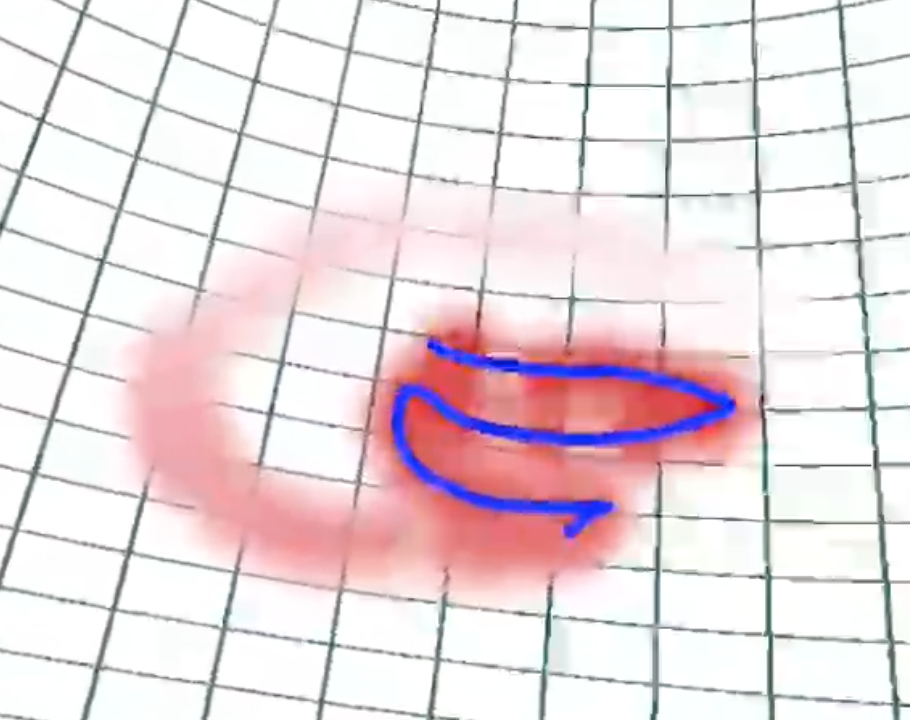
\includegraphics[width=\linewidth]{image_01.png}
\caption{Filtragem do cursor de VR. Amostras ruidosas em vermelho e valor filtrado em azul.}
\label{fig:filter01}
\end{figure}

\begin{figure}[h!]
\centering
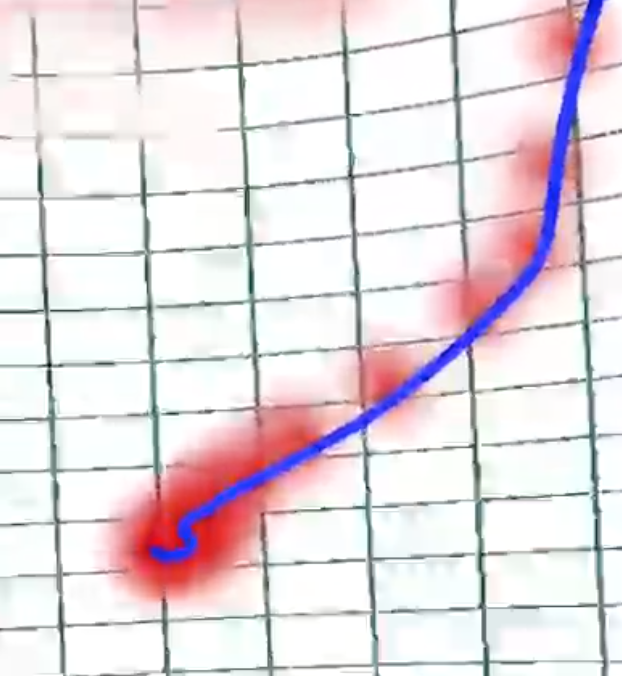
\includegraphics[width=\linewidth]{image_02.png}
\caption{Filtragem do cursor de VR. Amostras ruidosas em vermelho e valor filtrado em azul.}
\label{fig:filter02}
\end{figure}

\FloatBarrier % this prevents problems with misplaced pictures

A figura \ref{fig:chart_noise} mostra o gráfico da velocidade do curso ao longo da execução da aplicação. Ao comparar com o gráfico da figura \ref{fig:chart_filtered} gerado na mesma execução mas com o cursor filtrado, observamos que este último possui uma curva mais suave, indicando que o filtro de Kalman foi capaz de filtrar o ruído e assim suavizando o posicionamento capturado pelo controle.

\begin{figure}[h!]
\centering
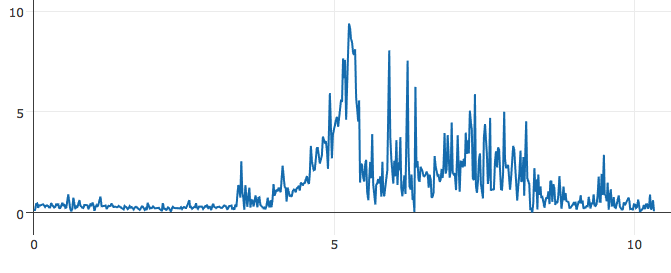
\includegraphics[width=\linewidth]{chart_noise.png}
\caption{Gráfico da velocidade do curso ao longo de uma execução da aplicação}
\label{fig:chart_noise}
\end{figure}

\begin{figure}[h!]
\centering
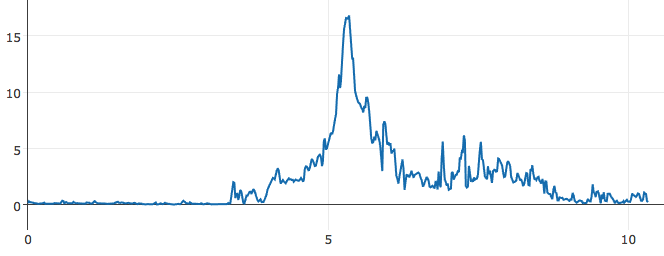
\includegraphics[width=\linewidth]{chart_filtered.png}
\caption{Gráfico da velocidade filtrada do curso ao longo de uma execução da aplicação}
\label{fig:chart_filtered}
\end{figure}
\FloatBarrier
%-------------------------------------------------------------------------------------------------
\section{Conclusão} \label{sec:conclusion}

Apresentou-se neste artigo a implementação do filtro de Kalman para estabilização do controle de realidade virtual da Oculus, o \textit{Gear VR Controller}. Concomitantemente, descreveu-se a visualização das entradas ruidosas fornecidas pelo controle e o efeito resultante após a aplicação do filtro. Apresentou-se também a implementação do jogo \textit{VRSnake} criado segundo a arquitetura de renderização baseada em \textit{shaders}.

Através dos resultados obtidos, verificou-se que a solução desenvolvida em \textit{Unity} para a aplicação do filtro foi efetivamente capaz de filtrar as posições ruidosas geradas pelo controlador e garantir um nível de controle mais estável em aplicações de realidade virtual. Da mesma maneira, o objetivo inicial de aliviar o trabalho de renderização atribuído à CPU foi alcançado por meio da distribuição de passos usualmente restritos à camada de aplicação para demais camadas da \textit{pipeline} gráfica.

% Trabalhos Futuros
Em trabalhos futuros, três passos são percebidos como cruciais. Em primeiro lugar, migrar inteiramente os processos da camada lógica para a camada de visualização, na unidade gráfica de processamento, com o propósito de permitir o controle e exibição de um número representativamente maior de serpentes. Em segundo lugar, aplicar aprendizagem de máquina nesta camada, objetivando-se um comportamento de busca e desvio de obstáculos (como outras serpentes e seu próprio corpo) mais inteligente, por conseguinte, desafiador. Por último, otimizar a performance objetivando maior fluidez.

\bibliographystyle{abbrv}
\bibliography{template}
\end{document}
